% Introductory presentation:intropres.tex

\documentclass{foils}
\usepackage{amsmath}
\usepackage{amssymb,latexsym}
\usepackage{graphicx}

\begin{document}
\title{A construction of complete-simple\\  
       distributive lattices}
\author{George~A. Menuhin\\
			Computer Science Department\\
         	University of Winnebago\\
         	Winnebago, MN 53714} 
\date{March 15, 2006}

\maketitle
\begin{abstract}
   In this presentation, we prove that there exist 
   \emph{complete-simple distributive lattices,} 
   that is, complete distributive lattices
   with only two complete congruences. 
\end{abstract}

\foilhead{The result}
%\section{Introduction}\label{S:intro} 
In this presentation, we prove the following result:

\begin{Theorem} 
There exists an infinite complete distributive 
lattice~$K$ with only the two trivial complete 
congruence relations.
\end{Theorem}

\foilhead{The construction}
%\section{The $\Pi^{*}$ construction}\label{S:P*} 
The following construction is crucial in the proof
of our theorem:

\begin{Definition}\label{D:P*} 
Let $D_{i}$, for $i \in I$, be complete distributive 
lattices satisfying condition~\textup{(J)}.  Their 
$\Pi^{*}$ product is defined as follows:
\[
   \Pi^{*} ( D_{i} \mid i \in I ) = 
   \Pi ( D_{i}^{-} \mid i \in I ) + 1;
\]
that is, $\Pi^{*} ( D_{i} \mid i \in I )$ is 
$\Pi ( D_{i}^{-} \mid i \in I )$ with a new 
unit element. 
\end{Definition}

\foilhead{}

\begin{figure}[hbt]
\centering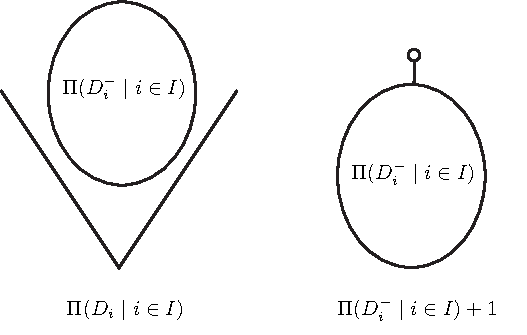
\includegraphics[scale=2]{products}
\caption{The product construction illustrated}\label{Fi:products}
\end{figure}

\foilhead{Notation}


If $i \in I$ and $d \in D_{i}^{-}$, then
\[
  \langle \dots, 0, \dots, d, \dots, 0, \dots \rangle
\]
is the element of\, $\Pi^{*} ( D_{i} \mid i \in I )$ whose 
$i$-th component is $d$ and all the other components 
are $0$.


See also Ernest~T. Moynahan, 1957.

\foilhead{Second result}

\begin{Theorem}\label{T:P*} 
Let $D_{i}$, $i \in I$, be complete distributive 
lattices satisfying condition~\textup{(J)}.  
Let $\Theta$ be a complete congruence relation on 
$\Pi^{*} ( D_{i} \mid i \in I )$. 
If there exist $i \in I$ and $d \in D_{i}$ with 
$d < 1_{i}$ such that, for all $d \leq c < 1_{i}$, 
\begin{equation*}\label{E:cong1} 
   \langle \dots, d, \dots, 0, \dots \rangle \equiv 
   \langle \dots, c, \dots, 0, \dots \rangle 
   \pod{\Theta}, 
\end{equation*}
then $\Theta = \iota$.
\end{Theorem}

\foilhead{Verification}

Since 
\begin{equation*}
\langle \dots, d, \dots, 0, \dots \rangle \equiv 
\langle \dots, c, \dots, 0, \dots \rangle 
\pod{\Theta}, 
\end{equation*}
and $\Theta$ is a complete congruence relation, 
it follows from condition~(J) that modulo $\Theta$
\begin{equation*}\label{E:cong}
 \langle \dots, d, \dots, 0, \dots \rangle \equiv
 \bigvee ( \langle \dots, c, \dots, 0, \dots \rangle 
 \mid d \leq c < 1 ). 
\end{equation*}

\foilhead{Verification completed}

Let $j \in I$, $j \neq i$, and let $a \in D_{j}^{-}$. 
Meeting both sides of the last congruence  
with $\langle \dots, a, \dots, 0, \dots \rangle$, 
we obtain that
\begin{equation*}
   0 = \langle \dots, a, \dots, 0, \dots \rangle 
     \pod{\Theta}, 
\end{equation*}
Using the completeness of $\Theta$ and the previous equation, 
we get:
\[
   0 \equiv \bigvee ( \langle \dots, a, \dots, 0, 
     \dots \rangle \mid a \in D_{j}^{-} ) = 1 
     \pod{\Theta}, 
\]
hence $\Theta = \iota$.

\foilhead{}

\begin{thebibliography}{9}

\bibitem{sF90}
Soo-Key Foo, 
\emph{Lattice Constructions}, 
Ph.D. thesis, 
University of Winnebago, Winnebago, MN, December, 1990.

\bibitem{gM68}
George~A. Menuhin, 
\emph{Universal Algebra}, 
D.~Van Nostrand, Princeton, 1968.

\bibitem{eM57}
Ernest~T. Moynahan, 
\emph{On a problem of M. Stone},
Acta Math. Acad. Sci. Hungar. \textbf{8} (1957), 
455--460.

\bibitem{eM57a}
Ernest~T. Moynahan, 
\emph{Ideals and congruence relations in lattices.} II,
Magyar Tud. Akad. Mat. Fiz. Oszt. K\"{o}zl. \textbf{9} 
(1957), 417--434.

\end{thebibliography}
\end{document}

